\documentclass[conference]{IEEEtran}
\IEEEoverridecommandlockouts
% The preceding line is only needed to identify funding in the first footnote. If that is unneeded, please comment it out.
\usepackage{amsmath,amssymb,amsfonts}
\usepackage{algorithmic}
\usepackage{graphicx}
\usepackage{textcomp}
\usepackage{xcolor}
\def\BibTeX{{\rm B\kern-.05em{\sc i\kern-.025em b}\kern-.08em
T\kern-.1667em\lower.7ex\hbox{E}\kern-.125emX}}
\begin{document}

    \title{Structured Attention Head Pruning in Decoder Transformers}

    \author{\IEEEauthorblockN{Welby Seely}
    \IEEEauthorblockA{\textit{Embedded AI Systems Lab} \\
    \textit{Eastern Michigan University}\\
    Ypsilanti, United States of America\\
    wseely@emich.edu}}

    \maketitle

    \begin{abstract}
        This paper proposes a framework for pruning the multi-head attention mechanism in decoder-based Large Language Models (LLMs).

        Unlike existing approaches, this attention head framework provides holistic analysis capabilities by integrating multiple evaluation metrics such as perplexity, energy consumption, evaluation time, and memory usage.

        As a proof-of-concept, the current methodology focuses on the Llama 3 8B architecture, performing layer-wise pruning and sensitivity analysis to measure the effects of approximating its attention mechanism.

        Results demonstrate potential savings in computational resources, highlighting specific layers as candidates for attention head approximation.
        Future work aims to extend this framework to additional components and model architectures.
    \end{abstract}

    \begin{IEEEkeywords}
        Large Language Models (LLMs), attention mechanism, pruning, resource optimization, sensitivity analysis
    \end{IEEEkeywords}

    \section{Introduction}
    Large Language Model (LLM) power consumption is increasingly problematic for datacenters, with \textit{The Electric Power
    Research Institute} forecasting that data centers may see their electricity consumption double by
    2030~\cite{kindig2024}.

    Optimizing these models is key to reducing power consumption.
    The cornerstone of optimization is determining what you need, and what you don't: determine the importance of
    aspects and components of the system, enabling you to perform systematic optimization with certainty.
    In Artificial Neural Networks (ANN), the atomic unit of these components is the artificial neuron.
    To optimize an ANN, understanding the sensitivity of the neuron to changes in its input and parameters is paramount,
    but the sheer size and complexity of LLMs makes this incredibly challenging.

    Sensitivity to pruning, the removal of neurons (weight matrix rows) is the initial phase of researching this sensitivity.
    Specifically, this work focuses on multi-head attention pruning in decoder transformers, introducing a structured framework for evaluating the impact of pruning on various model components.

    This research addresses limitations in the current literature, which often narrowly focus on specific metrics like perplexity and lack a unified framework for holistic analysis.

    By leveraging a multi-metric approach, we begin to explore the systemic effects of pruning, aiming to establish a more comprehensive understanding of parameter sensitivity in LLMs.

    \section{Related Works}

    An initial literature review was performed to identify gaps in the current research.
    Using Google Scholar\cite{GoogleScholar}, here are the gaps identified in the top 5 relevant works for the query ``llm pruning'':

    \begin{enumerate}
        \item Llm-pruner: On the structural pruning of large language models (2023)~\cite{ma2023llm}
        \begin{itemize}
            \item Does not support pruning the LLama3 architecture, misaligining query, key, and value vectors.
            \item Does not support the pruning of arbitrary heads.
            \item No measurement of per-token execution time and energy consumption.
        \end{itemize}
        \item LLM Pruning and Distillation in Practice: The Minitron Approach (2024)~\cite{sreenivas2024llm}
        \begin{itemize}
            \item Prunes the MLP hidden dimension, hidden dimension (embeddings), and layers.
            \item Does not support the pruning of arbitrary heads.
            \item No measurement of per-token execution time and energy consumption.
        \end{itemize}
        \item Everybody Prune Now: Structured Pruning of LLMs with only Forward Passes (2024)~\cite{dery2024everybodyprunenowstructured}
        \begin{itemize}
            \item Prunes heads, but does not measure sensitivity to the pruning of heads in different layers.
            \item No measurement of per-token execution time and energy consumption.
        \end{itemize}
        \item A Simple And Effective Pruning Approach For Large Language Models (2024) ~\cite{sun2024simpleeffectivepruningapproach}
        \begin{itemize}
            \item Prunes heads, but does not measure sensitivity to the pruning of heads in different layers.
            \item No measurement of per-token execution time and energy consumption.
        \end{itemize}
        \item Large Language Model Pruning (2024) ~\cite{huang2024largelanguagemodelpruning}
        \begin{itemize}
            \item Prunes heads, but does not measure sensitivity to the pruning of heads in different layers.
            \item No measurement of per-token execution time and energy consumption.
        \end{itemize}
    \end{enumerate}

    To conclude, this research fills a gap in current literature in the following ways:

    \begin{enumerate}
        \item Provides a framework to structurally prune all modules of a Decoder-based LLM
        \begin{itemize}
            \item Currently the Llama model is supported with Decoder Layer and Attention Head pruning implemented.
            \item All other layers will be eventually supported along with additional LLM models.
        \end{itemize}
        \item Supports structural pruning for grouped attention models.
        \item Records energy usage and execution time per token as fundamental metrics.
        \item Measures the holistic sensitivity of a Decoder-based LLM to the pruning of all modules.
    \end{enumerate}

    \section{Proposed Framework}
    This work proposes a structured framework, initially supporting the Llama 3 decoder architecture.
    The Huggingface Transformers library is used as a base for both pruning and evaluation of pruned and non-pruned
    (baseline) models~\cite{wolf2020huggingfacestransformersstateoftheartnatural}.

    The pruning framework enables the removal of arbitrary attention heads across arbitrary decoder layers,
    including associated key and value heads orphaned by pruning.
    For purposes of this proof-of-concept, the pruning methodology involves layer-wise removal of attention heads,
    measuring sensitivity of each layer to attention head pruning using four separate metrics.

    \subsection{Pruning Attention Heads for Group Query Attention Models}

    The Transformers library provides a de-facto abstract method, \textit{PreTrainedModel.prune\_heads}, for pruning a model's attention heads.
    This method is not implemented for many model types, including the Llama architecture.
    Implementing this method for the Llama 3 is particularly challenging due to its Grouped Query Attention architecture.

    The attention mechanism in LLMs is made up of 3 projected vectors: Query, Key, and Value vectors.
    Each vector can be divided into one or more attention heads: Query Heads (Q Heads), Key Heads, and Value Heads
    (often referred together as KV Heads.)
    These vectors are combined together in the Scaled Dot Product Attention operation ~\cite{vaswani2023attentionneed}.

    Grouped Query Attention (GQA) is an implementation of the attention mechanism that aims to combine the speed of
    the Multi-Query Attention (MQA) implementation and the quality of Multi-Head Attention (MHA) implementation.
    MQA shares a single KV head across all query heads; MHA has a single KV head per query head.
    GQA compromises by sharing a limited number KV heads between multiple query heads grouped together~\cite{ainslie2023gqatraininggeneralizedmultiquery}.

    Structural pruning was thus implemented based on query attention heads, eliminating KV Heads only if the entire Q Head group has been pruned.
    A visualization of this pruning is provided in figures~\ref{fig:gqa1},~\ref{fig:gqa2},~\ref{fig:gqa3}.

    \begin{figure}[!htbp]
        \centerline{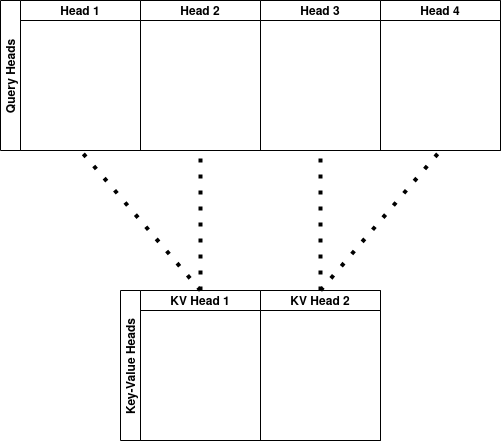
\includegraphics[width=0.66\columnwidth]{Unpruned GQA}}
        \caption{An unpruned GQA with 2 Groups.}
        \label{fig:gqa1}
    \end{figure}

    \begin{figure}[!htbp]
        \centerline{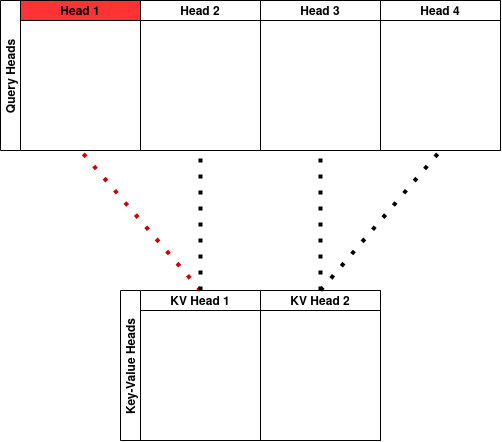
\includegraphics[width=0.66\columnwidth]{Pruned GQA 1}}
        \caption{A pruned GQA, with 1 attention head pruned.}
        \label{fig:gqa2}
    \end{figure}

    \begin{figure}[!htbp]
        \centerline{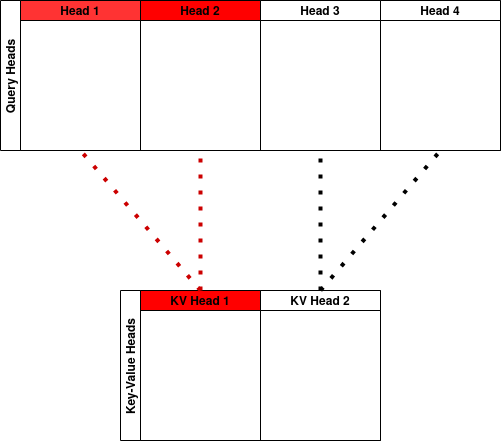
\includegraphics[width=0.66\columnwidth]{Pruned GQA 2}}
        \caption{A pruned GQA, with an entire group pruned, allowing the removal of a KV head.}
        \label{fig:gqa3}
    \end{figure}
    \clearpage

    \subsection{The Four Key Metrics}

    The framework evaluates the effects of multi-head attention pruning across four key metrics:

    \begin{enumerate}
        \item Perplexity
        \begin{itemize}
            \item Formally:
            \\
            \begin{equation}
                PP(p) = 2^{H(p)} = 2^{-\sum_x p(x) \log_2 p(x)}
                \label{eq:perplexity}
            \end{equation}
            \\
            Where \textit{H(p)} is the entropy of the probability distribution \textit{p}, \textit{p(x)} is the probability of a given token, and \textit{x} ranges over the vocabulary of the model.
            \item This is the model's confidence in its predicted tokens, lower values are better~\cite{jelinek1977perplexity}.
            \item Comparison to baseline:
            \\
            \begin{equation}
                \frac{PP_{baseline}}{PP_{pruned}}
                \label{eq:perplexity_comparison}
            \end{equation}
        \end{itemize}
        \item Energy consumption per token
        \begin{itemize}
            \item Measured using Nvidia's pynvml library~\cite{nvidia_ml_py}, captured in milli-joules.
            \item Comparison to baseline:
            \\
            \begin{equation}
                \frac{W_{pruned}}{W_{baseline}}
                \label{eq:energy_comparison}
            \end{equation}
        \end{itemize}
        \item Evaluation time per token
        \begin{itemize}
            \item Comparison to baseline:
            \\
            \begin{equation}
                \frac{T_{pruned}}{T_{baseline}}
                \label{eq:evaluation_time_comparison}
            \end{equation}
        \end{itemize}
        \item Allocated memory usage
        \begin{itemize}
            \item This is the static memory allocated to the model and its parameters.
            \item Fetched using \textit{torch.cuda.memory\_allocated()}
            \item Comparison to baseline:
            \\
            \begin{equation}
                \frac{M_{pruned}}{M_{baseline}}
                \label{eq:memory_time_comparison}
            \end{equation}
        \end{itemize}
    \end{enumerate}

    Sensitivity scores are calculated by comparing the performance of pruned layers against an unpruned baseline, allowing for a detailed analysis of which layers and components are more resilient to pruning.

    \section{Experimental Setup}
    The framework was tested on the Llama 3 8B model, consisting of 32 decoder layers and 32 attention heads per layer with a group size of 4~\cite{grattafiori2024llama3herdmodels}.

    The dataset used for evaluation was wikitext-2-v1~\cite{merity2016pointersentinelmixturemodels}.
    Each layer was assessed with a batch size of 5 across 25 prompts, running on an RTX 4090 GPU with the desktop environment disabled.
    The only process accessing CUDA during the test was the pruning framework, verified using the \textit{nvidia-smi} command line tool~\cite{nvidia_smi}.
    Persistence mode was enabled using \texit{nvidia-smi} to ensure the driver was not unloaded mid-test.

    Metrics were captured on a per-layer basis under two conditions: pruning all attention heads, and pruning every other attention head, the results averaged together.
    This is a rudimentary combination designed to gain an understanding of per-layer sensitivity within time-constraints: future tests will be more comprehensive, using progressive attention head pruning to collect more comprehensive metrics on a per-layer basis with the grain of the attention head.

    \section{Results and Discussion}
    \subsection{Perplexity}
    Perplexity measurements revealed that early layers were the most sensitive to pruning, with the first layer exhibiting over a 25\% degradation in perplexity compared to the baseline. Layers 20 through 28 were identified as good candidates for approximation due to their lower sensitivity.

    \subsection{Energy Consumption and Evaluation Time}
    Energy consumption per token decreased progressively with layer index, aligning with trends in evaluation time per token. This correlation suggests that later layers may offer significant energy and time savings when approximated.

    \subsection{Memory Usage}
    Allocated memory usage remained consistent across all layers, with negligible fluctuations attributed to noise. This indicates that the framework's pruning strategy maintains parameter efficiency.

    \section{Future Work}
    Future work includes enabling head pruning based on different strategies, measuring progressive pruning effects, generating heatmaps for head-level sensitivity, and expanding the framework to support additional components and architectures. This will provide deeper insights into the interactions between components and allow for broader applicability.

    \section*{Acknowledgment}
    The author would like to thank the Dr. Ourania Spantidi from the Embedded AI Systems Lab for her support and feedback in conducting this study.

    \bibliography{bibliography}
    \bibliographystyle{IEEEtran}

\end{document}
